\documentclass[11pt]{article}
\usepackage{geometry, titlesec}
\usepackage[parfill]{parskip}
\usepackage[italicdiff]{physics}
\usepackage{amsfonts, amsthm}
\usepackage[cm]{fullpage}
\usepackage{fancyhdr}
\usepackage{xcolor}
\usepackage{siunitx, graphicx}
\usepackage{enumitem}


\renewcommand{\footrulewidth}{.2pt}
\pagestyle{fancy}
\fancyhf{}
\lhead{Homework 1}
\rhead{Physics 133-B}
\setlength{\headheight}{11pt}
\setlength{\headsep}{11pt}
\setlength{\footskip}{24pt}
\lfoot{\today}
\rfoot{\thepage}


\titleformat{\section}[runin]{\normalfont\large\bfseries}{Problem \thesection.}{1em}{}
\titleformat{\subparagraph}[leftmargin]{\normalfont\large\bfseries}{}{0pt}{}

\setenumerate[1]{label={(\alph*)}}


\newcommand{\refeq}[1]{(\ref{#1})}

\newcommand{\beq}{\begin{equation*}}
\newcommand{\eeq}{\end{equation*}}

\newcommand{\beqn}{\begin{equation}}
\newcommand{\eeqn}{\end{equation}}

\newcommand{\qimplies}{\quad \implies \quad}


\newenvironment{statement}[1]
{
	\section{#1}
	\ignorespaces
}

\newenvironment{solution}
{
    \paragraph{Solution.}
    \ignorespaces
}




\DeclareSIUnit{\mph}{mph}


\begin{document}

\newcommand{\dist}{\SI{2}{\meter}}
\newcommand{\freq}{\SI{800}{\Hz}}
\newcommand{\vsound}{\SI{344}{\meter\per\second}}


\begin{statement}{}	% Y&F 16.61
	Consider two speakers emitting sound at the same volume with frequency $f = \freq$.  One speaker is located at the origin, and the other on the $y$ axis at $y = \dist$.  At what locations on the positive $x$ axis is the interference completely constructive?  At what points is it completely destructive?
	
	Now we decrease $f$ until there are no longer any points of completely destructive interference on the positive $x$ axis.  How low must $f$ be for this to occur?
\end{statement}



\newcommand{\lam}{\lambda}
\newcommand{\ddA}{d_A}
\newcommand{\ddB}{d_B}
\newcommand{\Dely}{\Delta y}
\newcommand{\wavel}{\SI{0.43}{\meter}}

\begin{solution}
	Consider the setup shown below:
	
	\begin{center}
		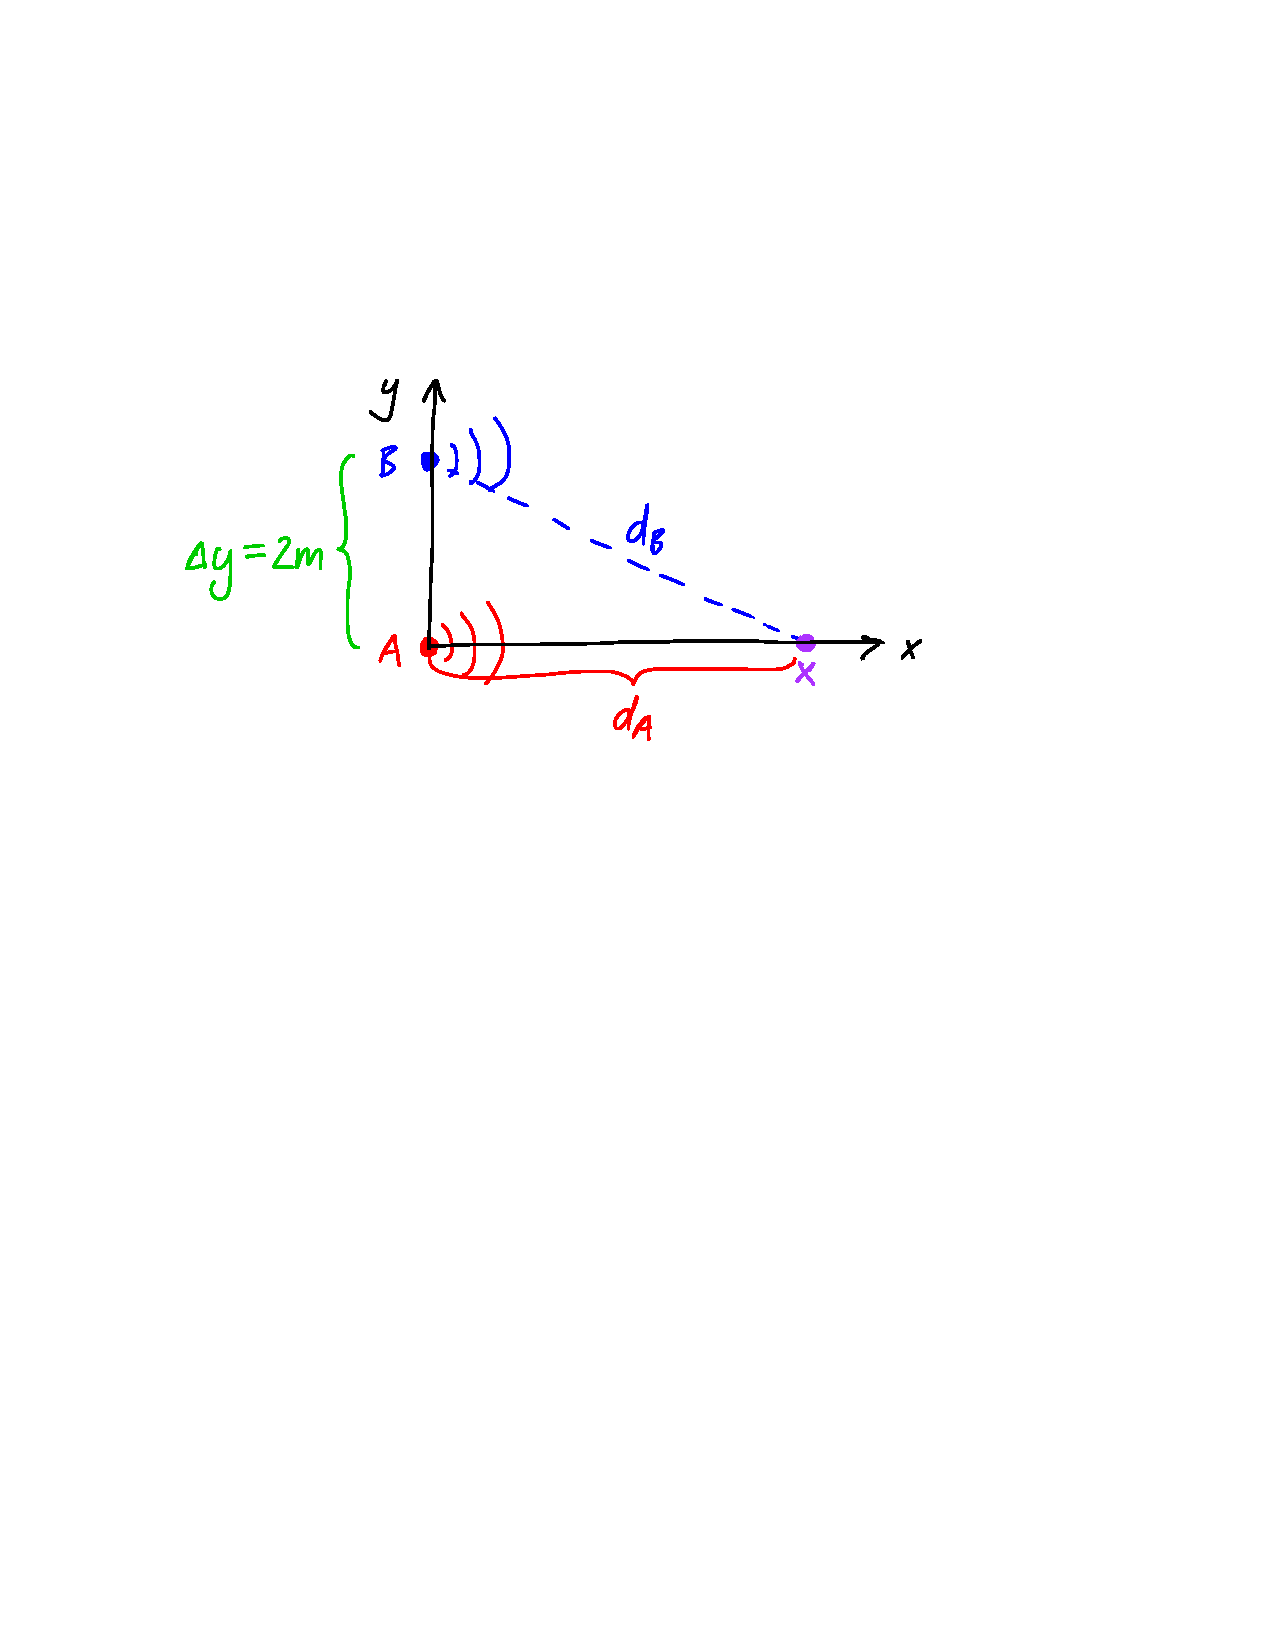
\includegraphics{fig1}
	\end{center}
	
	The path difference $d$ (which is called $\Delta x$ in the lecture slides) is given by
	\beq
		d = \ddB - \ddA = \ddA - x,
	\eeq
	and from trigonometry,
	\beq
		\ddB^2 = x^2 + (\Dely)^2
		\qimplies
		\ddB = \sqrt{x^2 + (\Dely)^2},
	\eeq
	where $\Dely$ is the distance between the two speakers.  Putting these together, we can write
	\beq
		d = \sqrt{x^2 + (\Dely)^2} - x.
	\eeq
	Completely constructive interference occurs where the interference pattern of the speakers has a maximum, which is when
	\begin{align*}
		d &= n \lam, &
		n &= 0, \pm 1, \pm 2, \ldots.
	\end{align*}
	Completely destructive interference occurs where it has a minimum, and
	\begin{align*}
		d &= \left( n + \frac{1}{2} \right) \lam, &
		n &= 0, \pm 1, \pm 2, \ldots.
	\end{align*}
	Recall that the wavelength $\lam = v / f$, where $v = \vsound$ is the speed of sound in air.  For this problem,
	\beq
		\lam = \frac{\vsound}{\freq}
		= \wavel.
	\eeq
	
	Constructive interference will occur at $x$ when
	\beq
		n \lam = \sqrt{x^2 + (\Dely)^2} - x.
	\eeq
	Solving for $x$,
	\beq
		\left( x + n \lam \right)^2 = x^2 + (\Dely)^2
		\qimplies
		x^2 + n \lam x + n^2 \lam^2 = x^2 + (\Dely)^2
		\qimplies
		n \lam x = (\Dely)^2 - n^2 \lam^2,
	\eeq
	which implies
	\beqn \label{const}
		x = \frac{(\Dely)^2}{n \lam} - n \lam.
	\eeqn
	Now we can plug in numerical quantities and $n = 0, \pm 1, \pm 2, \ldots$ into Eq.~\refeq{const} to find
	\begin{align*}
		x(n = 1) &= \frac{(\dist)^2}{\wavel} - (\wavel)
		= {\color{blue} \SI{8.87}{\meter}}, \\
		x(n = 2) &= \frac{(\dist)^2}{2 (\wavel)} - 2 (\wavel)
		= {\color{blue} \SI{3.79}{\meter}}, \\
		x(n = 3) &= \frac{(\dist)^2}{3 (\wavel)} - 3 (\wavel)
		= {\color{blue} \SI{1.81}{\meter}}, \\
		x(n = 4) &= \frac{(\dist)^2}{4 (\wavel)} - 4 (\wavel)
		= {\color{blue} \SI{0.61}{\meter}}.
	\end{align*}
	Note that $x$ is undefined for $n = 0$ and is negative for $n > 4$.  Plugging in $n = -1, -2, -3, \ldots$ would also give us negative values.  None of these makes sense since we are interested only in the positive $x$ axis.  
	
	For destructive interference, we have to satisfy
	\beq
		\left( n + \frac{1}{2} \lam \right) = \sqrt{x^2 + (\Dely)^2} - x,
	\eeq
	and solving for $x$ in the same manner as before gives us
	\beqn \label{dest}
		x = \frac{(\Dely)^2}{(n + 1/2) \lam} - \left( n + \frac{1}{2} \right) \lam.
	\eeqn
	Plugging in numerical quantities and $n = 0, 1, 2, \ldots$ into Eq.~\refeq{dest},
	\begin{align*}
		x(n = 0) &= \frac{(\dist)^2}{(1/2) (\wavel)} - \frac{1}{2} (\wavel)
		= {\color{blue} \SI{18.4}{\meter}}, \\
		x(n = 1) &= \frac{(\dist)^2}{(3/2) (\wavel)} - \frac{3}{2} (\wavel)
		= {\color{blue} \SI{5.56}{\meter}}, \\
		x(n = 2) &= \frac{(\dist)^2}{(5/2) (\wavel)} - \frac{5}{2} (\wavel)
		= {\color{blue} \SI{2.65}{\meter}}, \\
		x(n = 3) &= \frac{(\dist)^2}{(7/2) (\wavel)} - \frac{7}{2} (\wavel)
		= {\color{blue} \SI{1.15}{\meter}}, \\
		x(n = 4) &= \frac{(\dist)^2}{(9/2) (\wavel)} - \frac{9}{2} (\wavel)
		= {\color{blue} \SI{0.13}{\meter}}.
	\end{align*}
	Again, $x < 0$ for $n < 0$ and $n > 4$, which are not sensible.
	
	In order to find the frequency for which there is no destructive interference on the $x$ axis, we should look at $n = 0$, since this gives us the point with the largest value of $x$.  If we plug $n = 0$ into Eq.~\refeq{dest} and set $x = 0$, we are requiring that destructive interference can only occur at the origin.  Solving for the wavelength $\lam$ tells us the smallest wavelength at which there is still destructive interference.  We find
	\beq
		0 = \frac{(\Dely)^2}{\lam / 2} - \frac{\lam}{2}
		\qimplies
		\frac{\lam}{2} = \frac{(\Dely)^2}{\lam / 2}
		\qimplies
		\frac{\lam^2}{4} = (\Dely)^2
		\qimplies
		\lam = 2 \Dely.
	\eeq
	But if $\lam > 2 \Dely$, then
	\beq
		\frac{(\Dely)^2}{\lam / 2} < \frac{1}{2} \lam,
	\eeq
	and Eq.~\refeq{dest} tells us
	\beq
		x = \frac{(\Dely)^2}{\lam / 2} - \frac{1}{2} \lam < 0.
	\eeq
	This means there is no destructive interference on the $x$ axis.  Thus, we need to satisfy
	\beq
		\lam = \frac{v}{f} > 2 \Dely
		\qimplies
		f < \frac{v}{2 \Dely}.
	\eeq
	Plugging in numbers, we find
	\beq
		f < \frac{\vsound}{2 (\dist)}
		= {\color{blue} \SI{86}{\Hz}}.
	\eeq

\end{solution}




\clearpage

\newcommand{\ofreq}{\SI{10.5}{\giga\Hz}}
\newcommand{\ifreq}{\SI{12.5}{\giga\Hz}}
\newcommand{\pspeed}{\SI{35}{\meter\per\second}}
\newcommand{\sspeed}{\SI{30.6}{\meter\per\second}}

\begin{statement}{}	% Y&F 16.51
	A police car is waiting on the shoulder of Lake Shore Drive.  In order to catch speeding commuters, the officer uses a radar gun that emits sound of frequency {\ofreq}.  There is a single speeding car on the road, which is directly in front of or behind her.  When she fires the gun, the frequency that returns from the speeder's car is {\ifreq}.  What is the speed of the car?  Is it moving toward the officer, or away from her?

	A few moments later, the officers takes off at {\pspeed} in pursuit of the speeder, who does not change his speed.  If the officer fires the gun now, what frequency will she receive?
\end{statement}


\newcommand{\vL}{v_L}
\newcommand{\vS}{v_S}
\newcommand{\fL}{f_L}
\newcommand{\fS}{f_S}
\newcommand{\vcar}{v_\text{car}}
\newcommand{\voff}{v_\text{off}}

\begin{solution}
	This is a problem about the Doppler effect.  In general, we have
	\beqn \label{dopp}
		\fL = \frac{v \pm \vL}{v \pm \vS} \fS,
	\eeqn
	where $\fL$ and $\fS$ are the frequenceis in the frames of the listener and source, respectively, $\vL$ and $\vS$ are the velocities of the listener and source, and $v$ is the speed of sound.  (The speed of sound in air is $v = \vsound$.)  Written in this form, we choose a $+$ sign in the numerator if the listener is moving toward the source, and a $-$ sign if it is moving away.  The convention is flipped for the denominator: we choose a $-$ sign if the \emph{source} is moving toward the \emph{listener}, and a $+$ sign if it is moving away.
	
	It is easiest to answer the question about the direction of the car first.  Since the frequency that the officer hears is greater than the frequency she emitted, we know {\color{blue} the speeding car is moving toward her}.

	In order to find the speed of the car, we need to apply \refeq{dopp} twice.  Let $f$ be the {\ofreq} frequency emitted by the radar gun, and $f'$ the frequency that is ``heard'' by the speeding car.  Equation~\refeq{dopp} becomes
	\beqn \label{f}
		f' = \frac{v + \vcar}{v} f,
	\eeqn
	where $\vcar$ is the velocity of the speeding car, which is the ``listener'' in this scenario, and is moving toward the officer.  The officer, who is the ``source,'' is stationary.  Now we can use $f'$ to find the {\ifreq} frequency that returns to the officer, which we will call $f''$.  This is found by writing Eq.~\refeq{dopp} as
	\beqn \label{ff}
		f'' = \frac{v}{v - \vcar} f',
	\eeqn
	where the stationary officer is now the ``listener,'' and the speeding car is now the ``source,'' which again is moving toward the officer.
	
	Substituting Eq.~\refeq{f} into Eq.~\refeq{ff}, we find
	\beq
		f'' = \frac{v}{v - \vcar} \frac{v + \vcar}{v} f
		= \frac{v + \vcar}{v - \vcar} f.
	\eeq
	Now we can solve for $\vcar$:
	\beq
		f'' (v - \vcar) = f (v + \vcar)
		\qimplies
		(f'' - f) v = (f'' + f) \vcar
		\qimplies
		\vcar = \frac{f'' - f}{f'' + f} v.
	\eeq
	Finally, we can plug in known quantities to obtain
	\beq
		\vcar = \frac{(\ifreq) - (\ofreq)}{(\ifreq) + (\ofreq)} (\vsound)
		= \frac{2}{22.5} (\vsound)
		= {\color{blue} \sspeed},
	\eeq
	which is over \SI{68}{\mph}!  (The speed limit on Lake Shore Drive is 40--\SI{45}{\mph}.)
	
	When the officer pursues the car, the equivalent of Eq.~\refeq{f} is
	\beq
		f' = \frac{v - \vcar}{v - \voff} f,
	\eeq
	where $\voff$ is the speed of the officer's police car.  Here we use a $-$ sign in the numerator since the speeder is moving away from the officer, and a $-$ sign in the denominator because the officer is moving toward the speeder.  Likewise, the equivalent of Eq.~\refeq{ff} is
	\beq
		f'' = \frac{v + \voff}{v + \vcar} f'.
	\eeq
	Once again, we may substitute in $f'$ to find
	\beq
		f'' = \frac{v + \voff}{v + \vcar} \frac{v - \vcar}{v - \voff} f.
	\eeq
	Finally, plugging in quantities,
	\begin{align*}
		f'' &= \frac{(\vsound) + (\pspeed)}{(\vsound) + (\sspeed)} \frac{(\vsound) - (\sspeed)}{(\vsound) - (\pspeed)} (\ofreq)
		= \frac{379}{374.6} \frac{313.4}{309} (\ofreq) \\
		&= 1.03 (\ofreq)
		= {\color{blue} \SI{10.8}{\giga\Hz}}.
	\end{align*}
\end{solution}

\end{document}